\documentclass[a4paper]{article}

\usepackage[LGR, T1]{fontenc}
\usepackage[utf8]{inputenc}
\usepackage[english, greek]{babel}
\usepackage{listings}
\usepackage{xcolor}
\usepackage{graphicx}
\usepackage{caption}
\usepackage{subcaption}
\usepackage{float}
\graphicspath{ {./screenshots/} }

\definecolor{codegreen}{rgb}{0,0.6,0}
\definecolor{codegray}{rgb}{0.5,0.5,0.5}
\definecolor{codepurple}{rgb}{0.58,0,0.82}
\definecolor{backcolour}{rgb}{0.95,0.95,0.92}

\lstdefinestyle{mystyle}{
    backgroundcolor=\color{backcolour},   
    commentstyle=\color{codegreen},
    keywordstyle=\color{magenta},
    numberstyle=\tiny\color{codegray},
    stringstyle=\color{codepurple},
    basicstyle=\ttfamily\footnotesize,
    breakatwhitespace=false,         
    breaklines=true,                 
    captionpos=b,                    
    keepspaces=true,                 
    numbers=left,                    
    numbersep=5pt,                  
    showspaces=false,                
    showstringspaces=false,
    showtabs=false,                  
    tabsize=2
}

\lstset{style=mystyle}

\title{Προαιρετική Εργασία σε \textlatin{Python} 2019 - 2020}
\author{Θωμάς Γεώργιος, 1059634}
\date{2020}


\begin{document}
\maketitle

\begin{abstract}
Στην παρούσα εργασία με τη χρήση της \textlatin{Python} πραγματοποιήθηκε κατέβασμα και αποθήκευση αρχείων από το διαδίκτυο. Ύστερα, έγινε εξαγωγή των απαραίτητων στοιχείων από τα αρχεία αυτά σε μια βάση δεδομένων. Από εκεί, έγινε επεξεργασία και υπολογίστηκαν οι τελικές τιμές των ζητουμένων. Από τις τιμές αυτές πραγματοποιήθηκε εξαγωγή διαγραμμάτων αλλά και των \textlatin{csv} αρχείων.
\end{abstract}


\section*{Εισαγωγή}
Η εργασία αυτή πραγματοποιήθηκε σε λειτουργικό \textlatin{Linux} και συγκεκριμένα σε \textlatin{Ubuntu 18.04}. Έγινε χρήση της \textlatin{Python 3.6.9}. Ως \textlatin{text editor} χρησιμοποιήθηκε το \textlatin{Visual Studio Code} και ως βάση δεδομένων η \textlatin{SQLite}. Επιπλέον, για την πραγματοποίηση της εργασίας χρησιμοποιήθηκαν και οι κατάλληλες βιβλιοθήκες, οι οποίες φαίνονται στην αρχή του κάθε αρχείου. Τέλος, μέσα στον κώδικα υπάρχουν σχόλια καθώς και συναρτήσεις εκτύπωσης για την καλύτερη κατανόηση του προγράμματος.


\section{Κατέβασμα, αποθήκευση αρχείων και εξαγωγή δεδομένων}
Στον παρακάτω κώδικα υλοποιήθηκαν δύο συναρτήσεις. Η πρώτη κατεβάζει και αποθηκεύει τα αρχεία στον υπολογιστή. Με τη χρήση βιβλιοθηκών γίνεται σύνδεση στην ιστοσελίδα. Από εκεί αναζητείται το \textlatin{download link} με βάση τον τίτλο του, γίνεται κατέβασμα και ύστερα αποθήκευση. Οι πληροφορίες που χρειάζονται για να απαντηθούν τα ερωτήματα βρίσκονται όλες στα τέσσερα αρχεία που κατεβάζονται. Η δεύτερη συνάρτηση που υλοποιείται είναι αυτή για την εξαγωγή των απαραίτητων τιμών σε μία βάση δεδομένων αφού πρώτα φιλτραριστούν και κρατηθούν μόνο αυτά που χρειάζονται.

\selectlanguage{english}

\begin{lstlisting}[language=Python, caption=files.py]
from bs4 import BeautifulSoup # Scrap urls from webpages
import urllib.request # Make url requests
import requests # Open and store files from urls
import calendar # Get the months
import sqlite3 # Manage a database
import xlrd # Read excel files
import os # Manage directories
import re # Regeular expressions


# Download and store excel files
def download():
    # The main url to get download links
    main_url = "https://www.statistics.gr/en/statistics/-/publication/STO04/201X-Q4"

    for year in range(1, 5):
        new_url = main_url.replace("X", str(year)) # Change the year

        file_name = new_url.split("/")[-1] + ".xls" # Get the file name
        print("Downloading " + file_name + "...")
        
        # Open the corresponding page
        html_page = urllib.request.urlopen(new_url)

        # Parse the page
        soup = BeautifulSoup(html_page, "html.parser")

        # Find the first "a" tag with the given text
        link = soup.find("a", text="Arrivals of non-residents from abroad, by country of residence and by means of transport ")

        # Get the download link from the page
        url = link.get("href")

        # Get the relative path filename in respect to cwd
        rel_path_filename = "../" + "excel_files" + "/" + file_name

        # Open the link, download the file and store it in the given folder
        r = requests.get(url, allow_redirects=True)
        open(rel_path_filename, "wb+").write(r.content)

    print("All files downloaded.")


# Export the necessary information from excel files to database
def export_to_db():
    print("Exporting to database...")

    # Create/connect to database
    conn = sqlite3.connect("../tourism.db")

    # All excel files
    excel_files = os.listdir("../excel_files/")

    c = conn.cursor()

    # Create table
    c.execute('''CREATE TABLE IF NOT EXISTS statistics
                (Country TEXT, Air REAL, Railway REAL, Sea REAL, Road REAL, Month TEXT, Year INTEGER, unique(Country, Month, Year))''')

    # For every excel file
    for excel_file in excel_files:

        path = "../excel_files/" + excel_file

        # Open the file and get the sheets
        book = xlrd.open_workbook(path)

        # For every sheet within excel file
        for i, sheet in enumerate(book.sheets()):
            shown = 0
            # Get the first table of the sheet and add it to database
            for row_num in range(sheet.nrows):
                    row_value = sheet.row_values(row_num)
                    if row_value[0] == " - EUROPEAN UNION":
                        shown += 1
                    r = re.compile(r"\d.")
                    if shown == 1 and r.match(row_value[0]):
                        c.execute("INSERT INTO statistics VALUES (?, ?, ?, ?, ?, ?, ?)", 
                                 (row_value[1], row_value[2], row_value[3], row_value[4], row_value[5], calendar.month_name[i+1], excel_file.split("-")[0]))
                    if shown == 2:
                        break
    
    # Fix empty values
    means_of_transport = ["Air", "Railway", "Sea", "Road"]
    for mean in means_of_transport:
        c.execute("UPDATE statistics SET {} = 0 WHERE {} = ''".format(mean, mean))


    conn.commit() # Commit changes

    conn.close() # Close connection

    print("Done.")

\end{lstlisting}

\selectlanguage{greek}

Τα αποτελέσματα ύστερα από την εκτέλεση των συναρτήσεων αυτών είναι η αποθήκευση των αρχείων στον υπολογιστή και η δημιουργία της βάσης δεδομένων από τα αρχεία αυτά, όπως φαίνονται στα παρακάτω \textlatin{screenshots}. 

\begin{figure}[h]
\centering
\begin{subfigure}[b]{0.48\textwidth}
\centering

\includegraphics{files} 
\caption{Αρχεία \textlatin{Excel}}
\label{fig:excel_files}
\end{subfigure}
\hfill
\begin{subfigure}[b]{0.48\textwidth}
\centering

\includegraphics{database}
\caption{Βάση Δεδομένων}
\label{fig:database}
\end{subfigure}

\caption{Αρχεία που δημιουργήθηκαν}
\label{fig:all_files}
\end{figure}



\section{Επεξεργασία δεδομένων και εξαγωγή αποτελεσμάτων σε αρχεία \textlatin{csv}}

Στον παρακάτω κώδικα υλοποιήθηκαν πέντε συναρτήσεις. Στις τέσσερις από αυτές φορτώνονται τα δεδομένα από την βάση και επεξεργάζονται ώστε σαν αποτελέσματα να περιέχουν την πληροφορία που αφορά το κάθε ερώτημα. Η επεξεργασία των δεδομένων έγινε με την χρήση της βιβλιοθήκης \textlatin{pandas}. Η πέμπτη συνάρτηση εξάγει και αποθηκεύει τα τελικά δεδομένα σε μορφή \textlatin{csv}.

\selectlanguage{english}

\begin{lstlisting}[language=Python, caption=dataframe.py]
import pandas as pd # Analyze data
import calendar # Get the months
import sqlite3 # Manage the datatbase


def total_arrivals():
    print("Calculating Total Arrivals...")

    # Connect to database
    conn = sqlite3.connect("../tourism.db")

    # Get the dataframe from the database
    df = pd.read_sql_query("SELECT * FROM statistics", conn)
    
    # Get the total arrivals for each year
    total_df = pd.DataFrame({"Total Arrivals" : df.groupby(by = "Year")[["Air", "Railway", "Sea", "Road"]].sum().sum(axis=1)}).reset_index()

    # Close the connection
    conn.close()

    print("Done.")

    return total_df


def total_arrivals_by_country():
    print("Calculating Total Arrivals by Country...")

    # Connect to database
    conn = sqlite3.connect("../tourism.db")

    # Get the dataframe from the database
    df = pd.read_sql_query("SELECT * FROM statistics", conn)
    
    # Get the total arrivals for each year
    total_df = pd.DataFrame({"Total Arrivals" : df.groupby(by = "Country")[["Air", "Railway", "Sea", "Road"]].sum().sum(axis=1)}).reset_index()
    
    # Sort values by total arrivals
    total_df = total_df.sort_values(by = ["Total Arrivals"], ascending = False).head(4)

    # Close the connection
    conn.close()

    print("Done.")

    return total_df


def total_arrivals_by_means_of_transport():
    print("Calculating Total Arrivals by Means of Transport...")

    # Connect to database
    conn = sqlite3.connect("../tourism.db")

    # Get the dataframe from the database
    df = pd.read_sql_query("SELECT * FROM statistics", conn)
    
    # Get the total arrivals for each year
    total_df = pd.DataFrame({"Total Arrivals" : df[["Air", "Railway", "Sea", "Road"]].sum()}).reset_index()

    # Rename the column
    total_df = total_df.rename(columns = {"index":"Means of Transport"})
    
    # Sort values by total arrivals
    total_df = total_df.sort_values(by = ["Total Arrivals"], ascending = False)

    # Close the connection
    conn.close()

    print("Done.")

    return total_df


def total_arrivals_by_quarter():
    print("Calculating Total Arrivals by Quarter...")

    # Connect to database
    conn = sqlite3.connect("../tourism.db")

    # Get the dataframe from the database
    df = pd.read_sql_query("SELECT * FROM statistics", conn)

    # Add quarter column
    df["Quarter"] = ""

    # Make the dataframe
    total_df = pd.DataFrame(df)

    # Update the quarter column
    for month in calendar.month_name:
        if month in calendar.month_name[1:4]:
            total_df.loc[total_df["Month"] == month, "Quarter" ] = "Q1"
        elif month in calendar.month_name[4:7]:
            total_df.loc[total_df["Month"] == month, "Quarter" ] = "Q2"
        elif month in calendar.month_name[7:10]:
            total_df.loc[total_df["Month"] == month, "Quarter" ] = "Q3"
        elif month in calendar.month_name[10:13]:
            total_df.loc[total_df["Month"] == month, "Quarter" ] = "Q4"

    # Get the total arrivals for each year's quarter
    total_df = pd.DataFrame({"Total Arrivals" : df.groupby(by = ["Year", "Quarter"])[["Air", "Railway", "Sea", "Road"]].sum().sum(axis=1)}).reset_index()

    print("Done.")

    return total_df


# Export csv file from pandas' dataframe
def export_to_csv(df, csv_name):
    print("Exporting " + csv_name + "...")
    csv_path = "../csv_files/" + csv_name # Path to store the csv file
    df.to_csv(csv_path, index = False) # Save the csv file
    print("Done.")

\end{lstlisting}

\selectlanguage{greek}

Τα αποτελέσματα ύστερα από την εκτέλεση των συναρτήσεων αυτών, είναι η επιστροφή των τελικών αποτελεσμάτων σε μορφή \textlatin{dataframe} καθώς και η εξαγωγή τους σε αρχεία \textlatin{csv}, όπως φαίνονται στα παρακάτω \textlatin{screenshots}.


\begin{figure}[h]
\centering
\begin{subfigure}[b]{0.48\textwidth}
\centering
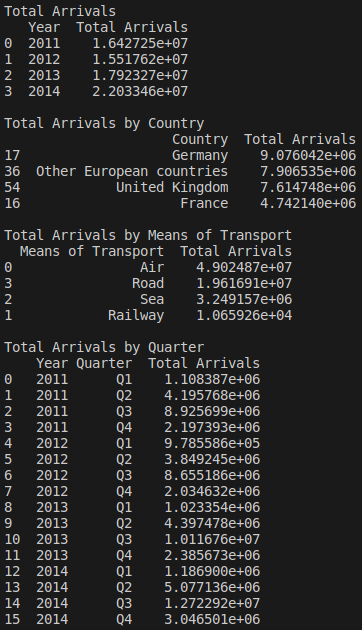
\includegraphics[scale=0.45]{dataframes} 
\caption{Εκτύπωση \textlatin{dataframes}}
\label{fig:print_dataframe}
\end{subfigure}
\hfill
\begin{subfigure}[b]{0.48\textwidth}
\centering
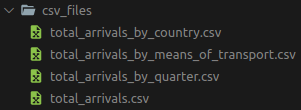
\includegraphics[scale=0.45]{csv}
\caption{Αρχεία \textlatin{csv}}
\label{fig:csv_files}
\end{subfigure}

\caption{Αποτελέσματα των συναρτήσεων}
\label{fig:dataframe_results}
\end{figure}


\section{Εξαγωγή διαγραμμάτων}
Στον παρακάτω κώδικα υλοποιήθηκαν τέσσερις συναρτήσεις. Η κάθε μία εξάγει γράφημα από το αντίστοιχο \textlatin{dataframe} του κάθε ερωτήματος. Με τη χρήση των βιβλιοθηκών \textlatin{pandas} και \textlatin{matplotlib} γίνεται κατάλληλο \textlatin{styling} για την καλύτερη κατανόηση των γραφημάτων και ύστερα αποθήκευση στον υπολογιστή.

\selectlanguage{english}

\begin{lstlisting}[language=Python, caption=diagram.py]
import matplotlib.pyplot as plt # Create diagrams
import pandas as pd # Analyze data
import textwrap as tw # Text wrapping

# Diagram for total arrivals
def export_total_arrivals(df, diagram_name):
    print("Exporting " + diagram_name + "...")
    rel_path_filename = "../diagrams/" + diagram_name
    df.plot(kind = "bar", x = "Year", y = "Total Arrivals", title = "Total Arrivals in 2011-2014", legend = False) # Plotting the dataframe
    plt.style.use("seaborn-dark") # Color style
    plt.ylabel("Total Arrivals") # Label for y axis
    plt.xlabel("Years") # Label for x axis
    plt.xticks(rotation = 0) # Rotation for x axis' labels
    plt.tight_layout() # Fit labels
    plt.savefig(rel_path_filename) # Save the diagram
    print("Done.")


# Diagram for total arrivals by country
def export_total_arrivals_by_country(df, diagram_name):
    print("Exporting " + diagram_name + "...")
    rel_path_filename = "../diagrams/" + diagram_name
    df.plot(kind = "bar", x = "Country", y = "Total Arrivals", title = "Total Arrivals by Country in 2011-2014", legend = False) # Plotting the dataframe
    plt.style.use("seaborn-dark") # Color style
    plt.ylabel("Total Arrivals") # Label for y axis
    plt.xlabel("Countries") # Label for x axis

    text = '''\
    Note: Other European Countries are European countries besides Austria, Belgium, Bulgaria, Denmark, Estonia, Ireland, 
    Spain, Italy, Croatia, Cyprus, Latvia, Lithuania, Luxembourg, Malta, Netherlands, Hungary, Poland, Portugal, 
    Romania, Slovakia, Slovenia, Sweden, Czech Republic, Finland, Albania, Switzerland, Norway, Iceland, Russia, Servia.
    '''

    # Format the text
    fig_txt = tw.fill(tw.dedent(text.rstrip()), width=80)

    # Place the text
    plt.figtext(0.5, -0.12, fig_txt, horizontalalignment = "center",
                fontsize = 8, multialignment = "left",
                bbox=dict(boxstyle = "round", facecolor = "#D8D8D8",
                        ec = "0.5", pad = 0.5, alpha = 1), fontweight = "bold")

    plt.xticks(rotation = 45) # Rotation for x axis' labels
    plt.tight_layout() # Fit labels
    plt.savefig(rel_path_filename, bbox_inches = "tight") # Save the diagram
    print("Done.")



# Diagram for total arrivals by means of transport
def export_total_arrivals_by_means_of_transport(df, diagram_name):
    print("Exporting " + diagram_name + "...")
    rel_path_filename = "../diagrams/" + diagram_name
    df.plot(kind = "bar", x = "Means of Transport", y = "Total Arrivals", title = "Total Arrivals by Means of Transport in 2011-2014", legend = False) # Plotting the dataframe
    plt.style.use("seaborn-dark") # Color style
    plt.ylabel("Total Arrivals") # Label for y axis
    plt.xlabel("Means of Transport") # Label for x axis
    plt.xticks(rotation = 0) # Rotation for x axis' labels
    plt.tight_layout() # Fit labels
    plt.savefig(rel_path_filename) # Save the diagram
    print("Done.")


# Diagram for total arrivals by quarter
def export_total_arrivals_quarter(df, diagram_name):
    print("Exporting " + diagram_name + "...")
    rel_path_filename = "../diagrams/" + diagram_name
    df.pivot("Year", "Quarter", "Total Arrivals").plot(kind="bar", title = "Total Arrivals by Quarter in 2011-2014") # Plotting the dataframe
    plt.style.use("seaborn-dark") # Color style
    plt.ylabel("Total Arrivals") # Label for y axis
    plt.xlabel("Years") # Label for x axis
    plt.xticks(rotation = 0) # Rotation for x axis' labels
    plt.tight_layout() # Fit labels
    plt.savefig(rel_path_filename) # Save the diagram
    print("Done.")

\end{lstlisting}

\selectlanguage{greek}

Το αποτέλεσμα ύστερα από την εκτέλεση των συναρτήσεων αυτών είναι η εξαγωγή των τεσσάρων διαγραμμάτων που απαντούν στα αντίστοιχα ερωτήματα.

\begin{figure}[H]
\centering
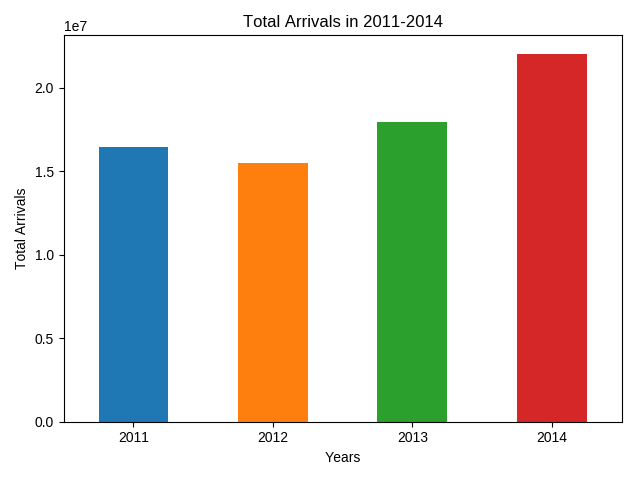
\includegraphics[scale=0.7]{total_arrivals} 
\caption{Συνολικές αφίξεις}
\label{fig:total_arrivals}
\end{figure}

\begin{figure}[H]
\centering
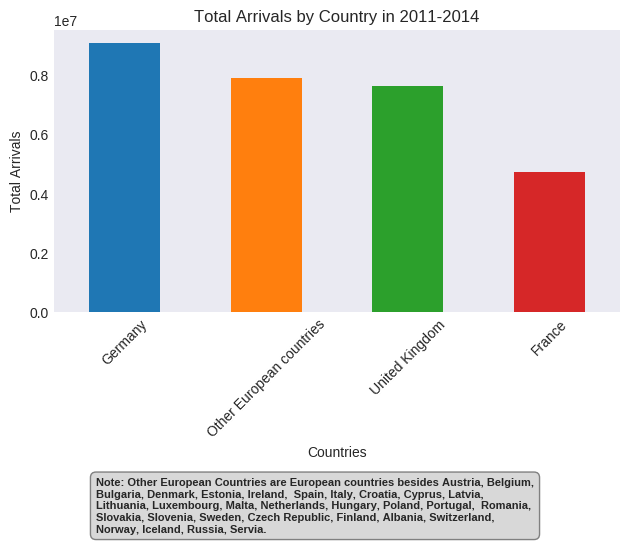
\includegraphics[scale=0.7]{total_arrivals_by_country}
\caption{Συνολικές αφίξεις ανά χώρα}
\label{fig:total_arrivals_by_country}
\end{figure}

\begin{figure}[H]
\centering
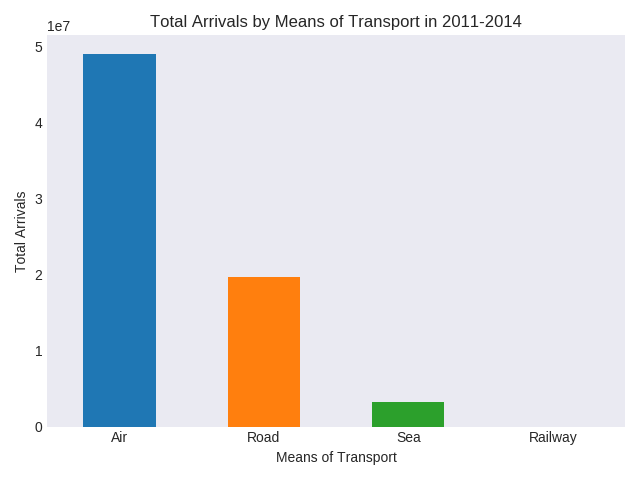
\includegraphics[scale=0.7]{total_arrivals_by_means_of_transport}
\caption{Συνολικές αφίξεις ανά μέσο μεταφοράς}
\label{fig:total_arrivals_by_means_of_transport}
\end{figure}

\begin{figure}[H]
\centering
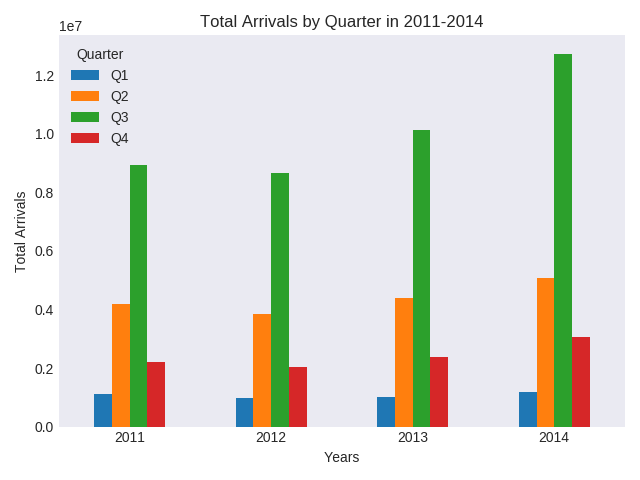
\includegraphics[scale=0.7]{total_arrivals_by_quarter}
\caption{Συνολικές αφίξεις ανά τρίμηνο}
\label{fig:total_arrivals_by_quarter}
\end{figure}

\section{Χρήση των συναρτήσεων για την εξαγωγή των αποτελεσμάτων}
Στον παρακάτω κώδικα καλούνται όλες οι συναρτήσεις με τα σωστά ορίσματα και τη σωστή σειρά έτσι ώστε να εξαχθούν τα ζητούμενα αποτελέσματα. Το αρχείο αυτό είναι το κύριο και είναι αυτό που χρειάζεται να εκτελεστεί για να παρθούν τα αποτελέσματα. Το αρχείο αυτό χρειάζεται να εκτελεστεί μία φορά. Αν εκτελεστεί πάνω από μία φορά θα βγάλει σφάλμα καθώς θα προσπαθήσει να εισάγει στη βάση ίδιες τιμές.

\selectlanguage{english}
\begin{lstlisting}[language=Python, caption=main.py]
import dataframe
import diagram
import files
import os

# Get this file directory and set it as cwd
dir_path = os.path.dirname(os.path.realpath(__file__))
os.chdir(dir_path)

files.download()

files.export_to_db()

# Total arrivals for each year
total_arrivals = dataframe.total_arrivals()
dataframe.export_to_csv(total_arrivals, "total_arrivals.csv")
diagram.export_total_arrivals(total_arrivals, "total_arrivals.png")

# Total arrivals by country
total_arrivals_by_country = dataframe.total_arrivals_by_country()
dataframe.export_to_csv(total_arrivals_by_country, "total_arrivals_by_country.csv")
diagram.export_total_arrivals_by_country(total_arrivals_by_country, "total_arrivals_by_country.png")

# Total arrivals by means of transport
total_arrivals_by_means_of_transport = dataframe.total_arrivals_by_means_of_transport()
dataframe.export_to_csv(total_arrivals_by_means_of_transport, "total_arrivals_by_means_of_transport.csv")
diagram.export_total_arrivals_by_means_of_transport(total_arrivals_by_means_of_transport, "total_arrivals_by_means_of_transport.png")

# Total arrivals by each year's quarter
total_arrivals_by_quarter = dataframe.total_arrivals_by_quarter()
dataframe.export_to_csv(total_arrivals_by_quarter, "total_arrivals_by_quarter.csv")
diagram.export_total_arrivals_quarter(total_arrivals_by_quarter, "total_arrivals_by_quarter.png")

\end{lstlisting}
\selectlanguage{greek}

Ύστερα από την εκτέλεση του κώδικα αυτού, εξάγονται τα αρχεία \textlatin{csv} και τα διαγράμματα, τα οποία έχουν παρουσιαστεί προηγουμένως. Στο παρακάτω \textlatin{screenshot} φαίνονται τα εκτυπωμένα μηνύματα του \textlatin{terminal}. 


\begin{figure}[H]
\centering
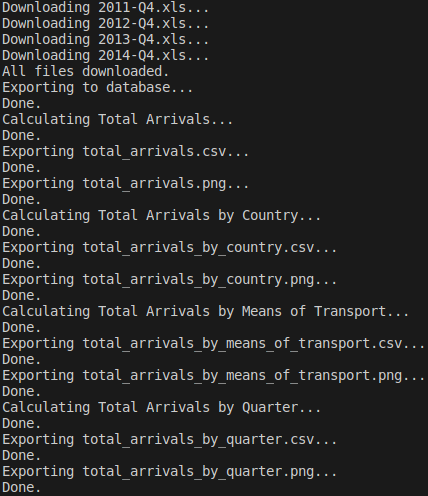
\includegraphics[scale=0.7]{terminal} 
\caption{Εκτύπωση Μηνυμάτων}
\label{fig:terminal}
\end{figure}

\end{document}
